%%%%%%%%%%%%%%%%%%%%%%%%%%%%%%%%%%%%%%%%%%%%%%%%%%%%%%%%%%%%%%%
%%%  NEF = NESS of a driven Ring, flutuations 
%%%%%%%%%%%%%%%%%%%%%%%%%%%%%%%%%%%%%%%%%%%%%%%%%%%%%%%%%%%%%%%

\documentclass[aps,prl,floats,floatfix,twocolumn]{revtex4}

% special 
\usepackage{ifthen}
\usepackage{ifpdf}
\usepackage{color}

\ifpdf
\usepackage{graphicx}
\usepackage{epstopdf}
\else
\usepackage{graphicx}
\usepackage{epsfig}
\fi
\graphicspath{{./Figs/}{./}}

% fonts
\usepackage{latexsym}
\usepackage{amsmath}
\usepackage{amssymb}
\usepackage{bm}
\usepackage{wasysym}

%\usepackage{hyperref}

%%%%%%%%%%%%%%%%%%%%%%%%%%%%%%%%%%%%%%%%%%%%%%%%%%%%%%%%%%%%%%%%

% NEW 
\newcommand{\abs}[1]{\left|#1\right|}
\newcommand{\Prob}{\mbox{Prob}\,}
\newcommand{\erf}{\mbox{erf}\,}
\newcommand{\df}{{\rm d}}

% math symbols I
\newcommand{\sinc}{\mbox{sinc}}
\newcommand{\const}{\mbox{const}}
\newcommand{\trc}{\mbox{trace}}
\newcommand{\intt}{\int\!\!\!\!\int }
\newcommand{\ointt}{\int\!\!\!\!\int\!\!\!\!\!\circ\ }
\newcommand{\ar}{\mathsf r}
\newcommand{\im}{\mbox{Im}}
\newcommand{\re}{\mbox{Re}}

% math symbols II
\newcommand{\eexp}{\mbox{e}^}
\newcommand{\bra}{\left\langle}
\newcommand{\ket}{\right\rangle}

% Mass symbol
\newcommand{\mass}{\mathsf{m}} 
\newcommand{\Mass}{\mathsf{M}} 

% more math commands
\newcommand{\tbox}[1]{\mbox{\tiny #1}}
\newcommand{\bmsf}[1]{\bm{\mathsf{#1}}} 
%\newcommand{\amatrix}[1]{\matrix{#1}} 
\newcommand{\amatrix}[1]{\begin{matrix} #1 \end{matrix}} 
\newcommand{\pd}[2]{\frac{\partial #1}{\partial #2}}

% equations
\newcommand{\mylabel}[1]{\label{#1}} 
%\newcommand{\mylabel}[1]{\textcolor{blue}{[#1]}\label{#1}} 
\newcommand{\beq}{\begin{eqnarray}}
\newcommand{\eeq}{\end{eqnarray}} 
\newcommand{\be}[1]{\begin{eqnarray}\ifthenelse{#1=-1}
{\nonumber}{\ifthenelse{#1=0}{}{\mylabel{e#1}}}}
\newcommand{\ee}{\end{eqnarray}} 

% arrangement
\newcommand{\drawline}{\begin{picture}(500,1)\line(1,0){500}\end{picture}}
\newcommand{\bitem}{$\bullet$ \ \ \ }
\newcommand{\Cn}[1]{\begin{center} #1 \end{center}}
\newcommand{\mpg}[2][1.0\hsize]{\begin{minipage}[b]{#1}{#2}\end{minipage}}
\newcommand{\mpgt}[2][1.0\hsize]{\begin{minipage}[t]{#1}{#2}\end{minipage}}
\newcommand{\sect}[1]{{\bf #1.-- }}


% more
%\newcommand{\Eq}[1]{Eq.\!\!~(\ref{#1})}
%\newcommand{\Fig}[1]{Fig.\!\!~\ref{#1}}  
\newcommand{\Eq}[1]{\textcolor{blue}{Eq.\!\!~(\ref{#1})}} 
\newcommand{\Fig}[1]{\textcolor{blue}{Fig.}\!\!~\ref{#1}} 
\newcommand{\hide}[1]{}
%\newcommand{\hide}[1]{\textcolor{red}{[hidden text]}} %{}
\newcommand{\rmrk}[1]{\textcolor{red}{#1}}
%\newcommand{\Rmrk}[1]{\textcolor{blue}{\LARGE\bf #1}}

%\renewcommand{\includegraphics}[2][]{\ \\ \ FIGURE: \ \\ \ }
\renewcommand{\cite}[1]{\textcolor{blue}{[\onlinecite{#1}}]} %{[\onlinecite{#1}]} 


%\def\circbul{{\bigcirc \mkern-8mu _{\bullet} \mkern-8mu}} 
%\newcommand{\overline}[1]{\overline{#1}}

%%%%%%%%%%%%%%%%%%%%%%%%%%%%%%%%%%%%%%%%%%%%%%%%%%%%%%%%%%%%%%%%%%%%%%%%%%%%%%%%%%%%%%%%%%
%%%%%%%%%%%%%%%%%%%%%%%%%%%%%%%%%%%%%%%%%%%%%%%%%%%%%%%%%%%%%%%%%%%%%%%%%%%%%%%%%%%%%%%%%%
 
\begin{document}

\title{Non-equilibrium steady state and induced currents of a mesoscopically-glassy system:\\
interplay of resistor-network theory and Sinai physics}

\author{Daniel Hurowitz$^1$, Saar Rahav$^2$, Doron Cohen$^1$}

\affiliation{
\mbox{$^1$Department of Physics, Ben-Gurion University of the Negev, Beer-Sheva, Israel} \\
\mbox{$^1$Schulich Faculty of Chemistry, Technion - Israel Institute of Technology, Haifa 32000, Israel}
}

\begin{abstract}
We introduce an explicit solution for the non-equilibrium steady state (NESS) 
of a ring that is coupled to a thermal bath, and is driven by an external 
hot source with log-wide distribution of couplings. 
Having time scales that stretch over several decades is similar to glassy systems.
Consequently there is a wide range of driving intensities where the NESS 
is like that of a random walker in a biased Brownian landscape. 
We investigate the resulting statistics of the induced current~$I$. 
For a single ring we discuss how $\text{sign}(I)$ fluctuates as the intensity 
of the driving is increased, while for an ensemble of rings we highlight 
the fingerprints of Sinai physics on the $\text{abs}(I)$ distribution.   
\end{abstract}

\maketitle


%%%%%%%%%%%%%%%%%%%%%%%%%%%%%%%%%%%%%%%%%%%%%%%%%%%%%%%%%%%%%%%%%%%%%%%%%

The transport in a chain due to random non-symmetric transition
probabilities
is a fundamental problem in statistical mechanics \cite{derrida,d1,d2,d3,d4}.
It can be regarded as {\em a random walk in a random environment} \cite{sinai,sinai2}. 
%
This type of dynamics is of great relevance for surface diffusion \cite{surface}, thermal
ratchets~\cite{brownian1,brownian2,brownian3,ratchets}  and was used to model
diverse biological systems, such as molecular motors, enzymes, and unidirectional motion 
of proteins along filaments \cite{motors1,brownian4,motors2,motors3}.
Of particular interest are applications that concern the conduction 
of DNA segments \cite{DNA1,DNA3}, and thin glassy electrolytes under high voltages 
\cite{Wichmann,Roling1,Roling2,Roling3,Roling4,Nitzan}.

Mathematically one can visualize the dynamics as a random-walk 
of a particle that makes incoherent jumps between ``sites" in a network.
In an unbounded quasi-one-dimensional network we might have either diffusion 
or sub-diffusive Sinai spreading \cite{sinai}, depending on whether the transitions rates 
form a symmetric matrix or not. In contrast, when the system is bounded 
% (and without disjoint components) 
it eventually reaches a well-defined steady state. 
This would be an equilibrium {\em canonical} state if the transition rates 
were detailed-balanced, else it is termed non-equilibrium steady state (NESS). 

We would like to consider the NESS of a mesoscopically glassy system.
By ``glassiness" we mean that the rates that are induced by a bath, 
or by an external source, have a log-wide distribution, 
hence many time scales are involved. 
Specifically we consider a common way of maintaining a NESS (\Fig{f0}):
a system that is coupled to a driving source (``hot bath") 
that spoils the detailed-balance of the environment (``cold bath"). 
The log wide distribution of the transition rates leads to a novel NESS.
% 
In previous publications we have pointed out that due to ``glassiness" 
(also termed ``sparsity") the physics of Sinai-type disorder is 
a relevant ingredient in the analysis of energy absorption \cite{kbb} 
and transport \cite{ner}.  
   

%%%%%%%%%%%%%%%%%%%%%%%%%%%
\begin{figure}
\includegraphics[width=7cm]{bath2}
\caption{
A ring made up of $N$ sites is immersed in a ``cold" bath 
and subjected to a ``hot" driving source \cite{images}. 
As a result a current is induced.  
%
In the numerics the the driving source induces 
rates that are log-box distributed over 6~decades. 
} 
\label{f0}
\end{figure}



%%%%%%%%%%%%%%%%%%%%%%%%%%%
\sect{Scope}
%
% 
Below we introduce an explicit NESS solution for a minimal model that 
has all the essential ingredients of the problem, involving transitions between sites on a ring 
and a log-wide distribution of couplings to an external driving source. 
The induced steady state current~$I$ is the central quantity used to characterize 
the NESS in actual experiments. The purpose of the present study is to investigate 
its statistics. Specifically, for a single ring we discuss how $\text{sign}(I)$ fluctuates    
as the intensity of the driving is increased, while for an ensemble 
of rings we highlight the fingerprints of Sinai physics on the $\text{abs}(I)$ distribution.  

%%%%%%%%%%%%%%%%%%%%%%%%%%%
\sect{Remarks}
%
% 
Previous study of Sinai-type disordered systems \cite{sinai2}, 
has considered an open geometry with uncorrelated transition rates 
that have the same coupling everywhere. Consequentially 
the random-resistor-network aspect (which is related to local 
variation of the couplings) has not emerged.
% 
%For the closed topology studied here the statistics of~$I$ are not only affected 
%by the wide distribution of transition rates but also by the random nature of 
%the affinity that drives the currents at steady state. This affinity, 
%which we call below {\em stochastic-motive-force} (SMF) is due to the mismatch 
%between the equilibrium distributions that would result if the system were coupled 
%only to the bath or to the driving source.  
%
Furthermore, in the physically motivated setup that we have 
defined above (ring+bath+driving) Sinai physics would not arise 
if the couplings to the driving source were merely disorderly random. 
The log-wide distribution is a crucial ingredient. 
%
Finally, in a closed (ring) geometry, unlike an open (two terminal) geometry, 
the statistics of~$I$ is not only affected by the distribution of transition rates, 
but also by the spatial profile of the NESS. 
This is like ``canonical" as opposed to ``grand canonical" setting, 
leading to remarkably different results.
 
\clearpage

%%%%%%%%%%%%%%%%%%%%%%%%%%%%%%%%%%%%%%%%%%%%%%%%%%%%%%%%%%%%%%%%%%%%%%%%%%%%%%%%%
%%%%%%%%%%%%%%%%%%%%%%%%%%%%%%%%%%%%%%%%%%%%%%%%%%%%%%%%%%%%%%%%%%%%%%%%%%%%%%%%%
\sect{The model}
%
%
Consider a ring that consists of sites labeled by~$n$ 
with positions ${x=n}$ that are defined modulo~$N$. 
The bonds are labeled as ${\overrightarrow{n}\equiv(n{-}1 \leadsto n)}$.
The inverse bond is $\overleftarrow{n}$, and if direction does 
not matter we label it $\bar{n}$. The position of the $n$th bond 
is defined as $x_n \equiv n{-}(1/2)$. The on-site energies $E_n$ 
are normally distributed over a range $\Delta$,  
and the transitions rates are between near-neighbor sites:   
%
\beq
w_{\overrightarrow{n}} \ \ = \ \ w^{\beta}_{\overrightarrow{n}} + \nu g_{\bar{n}}
\eeq 
%
Here $w^{\beta}$ are the rates that are induced by a bath that has 
a finite temperature $T_B$. The $g_{\bar{n}}$ are 
couplings to a driving source that has an intensity~$\nu$. 
These coupling are log-box distributed within ${[g_{\text{min}},g_{\text{max}}]}$.
This means that $\ln(g_{\bar{n}})$ are distributed uniformly 
over a range ${\sigma=\ln(g_{\text{max}}/g_{\text{min}})}$. 
%
The bath transition rates satisfy detailed-balance, 
namely $w^{\beta}_{\overrightarrow{n}}/w^{\beta}_{\overleftarrow{n}} = \exp[-(E_{n}{-}E_{n{-}1})/T_B]$.
The driving spoils the detailed-balance. We define the resulted 
stochastic field as follows:
%
\be{100}
\mathcal{E}(x_n) \ \equiv \ \ln \left[\frac{w_{\overrightarrow{n}}}{w_{\overleftarrow{n}}}\right] 
\ \approx \ - \left[ \frac{1}{1+g_{\bar{n}}\nu} \right] \frac{E_n{-}E_{n{-}1}}{T_B}
\ee
%
where the last equality assumes ${\Delta \ll T_B}$,  
and without loss of generality the $g_{\bar{n}}$ have been re-scaled 
such that all the bath-induced transitions have 
the same average transition rate ${\bar{w}^{\beta}=1}$. 


%%%%%%%%%%%%%%%%%%%%%%%%%%%
\sect{The direction of the current}
%
%
The stochastic motive force (SMF), also known as the affinity, 
or as the entropy production \cite{eprd1,eprd2,eprd3,eprd4}
determines $\text{sign}(I)$. It is defined as follows:
%
\be{101}
\mathcal{E}_{\circlearrowleft} 
\ \ \equiv \ \ \ln \left[\frac{ \prod_n w_{\overrightarrow{n}}}{ \prod_n w_{\overleftarrow{n}}}\right] 
\ \ = \ \ \oint \mathcal{E}(x) \, dx 
\ee
%
Using \Eq{e100} one observes that for ${\nu \ll g_{\text{max}}^{-1}}$ 
the SMF is linear ${\mathcal{E}_{\circlearrowleft}\propto \nu}$,  
while for ${\nu \gg g_{\text{min}}^{-1}}$ it vanishes ${\mathcal{E}_{\circlearrowleft}\propto 1/\nu}$.
In the intermediate regime, which we call below {\em the Sinai regime},  
the SMF changes sign several times, see \Fig{f2}. 
Using the notations
%
\be{1021}
\tau \ \ \equiv \ \ \frac{1}{\sigma}\ln(g_{\text{max}}\nu)
\eeq
% 
and $\tau_n = (1/\sigma)\ln(g_{\text{max}}/g_{\bar{n}})$,  
the expression for the SMF takes the following form:
%
\be{102}
\mathcal{E}_{\circlearrowleft}(\tau) = -\sum_{n=1}^N f_{\sigma}(\tau-\tau_n) \frac{E_n{-}E_{n{-}1}}{T_B}
\eeq 
%
where $f_{\sigma}(t)\equiv [1+\eexp{\sigma t}]^{-1}$ is like a step function.
If $f(t)$ were a sharp step function it would follows 
that in the Sinai regime $\mathcal{E}_{\circlearrowleft}(\tau)$ 
is formally like a random walk. 
The number of sign reversals equals the number of times 
the random walker cross the origin. We have here a coarse-grained 
random walk: the $\tau_n$ are distributed uniformly over a range ${[0,1]}$,  
and each step is smoothed by $f_{\sigma}(t)$ such that the 
effective number of coarse-grained steps is $\sigma$.  
Hence we expect the number of sign change to be not $\sim\sqrt{\pi N}$ \cite{rw1,feller}
but $\sim\sqrt{\pi \sigma}$, reflecting the log-width of the distribution.


%%%%%%%%%%%%%%%%%%%%%%%%%%%%%%%%%%%%%%%%%%
\sect{Adding bonds in series}
%
%
The NESS equations are quite simple and can be solved using elementary 
algebra as in \cite{Wichmann,Roling1,Nitzan,ner}, 
or optionally using the network formalism for stochastic systems \cite{net1,net2,net3}.
Below we propose a generalized resistor-network approach 
that allows to obtain a more illuminating version for the NESS, 
that will provide a better insight for the statistical analysis.  
Let us assume that we have a NESS with a current $I$. 
The steady state equations for two adjacent bonds are 
%
\beq
I &=& w_{\overrightarrow{1}} p_{0} - w_{\overleftarrow{1}}p_{1} \\
I &=& w_{\overrightarrow{2}} p_{1} - w_{\overleftarrow{2}}p_{2}
\ee
%
We can combine them into one equation: 
%
\beq
I = \overrightarrow{G} p_{0} - \overleftarrow{G} p_{2},  
\ \ \ \ \ 
\overrightarrow{G} \equiv 
\left[ \frac{1}{w_{\overrightarrow{1}}} + 
\frac{1}{w_{\overrightarrow{2}}} 
\left(\frac{w_{\overleftarrow{1}}}{w_{\overrightarrow{1}}}\right) \right]^{-1}
\eeq
%
and similar expression for $\overleftarrow{G}$. 
We can repeat this procedure iteratively.  If we 
have $N$ bonds in series we get
%
\beq
\overrightarrow{G} \  \ = \ \ \left[ \sum_{m=1}^N \frac{1}{w_{\overrightarrow{m}}} 
\,\exp\left(-\int_0^{m{-}1}\!\!\!\!\!\!\!\mathcal{E}(x)dx \right) \right]^{-1} 
\eeq
%
Coming back to the ring,  we can cut it at an arbitrary site~$n$, 
and calculate the associated $G$s. 
It follows that ${I=(\overrightarrow{G}_n- \overleftarrow{G}_n) \, p_{n}}$.
Consequently the NESS is
%
\beq
p_{n} \ \ = \ \ \frac{I}{\overrightarrow{G}_n- \overleftarrow{G}_n} 
\eeq
%
and  $I$ can be regarded as the normalization factor:
%
\beq
I \ = \ \left[\sum_{n=1}^N \frac{1}{\overrightarrow{G}_n-\overleftarrow{G}_n}\right]^{-1}
\eeq    
%
In the next paragraph we show how to write these results 
in an explicit way that illuminates the relevant physics. 



%%%%%%%%%%%%%%%%%%%%%%%%%%%%%%%%%%%%%%%%%%
\sect{The NESS formula}
%
%
We define the conductance of a bond as the geometric mean 
of the clockwise and anticlockwise transmission rates: 
%
\beq  
w(x_n) \ \ = \ \ \sqrt{ w_{\overrightarrow{n}} w_{\overleftarrow{n}} }
\eeq
%
Hence $w_{\overrightarrow{n}} = w(x_n) \exp[(1/2)\mathcal{E}(x_n)]$.
Accordingly 
%
%
\beq
\overrightarrow{G}_n = \left[ \sum_{m=n+1}^{N+n} \frac{1}{w(x_m)} 
\,\exp\left(-\int_{n}^{x_m} \!\!\!\mathcal{E}(x)dx \right) \right]^{-1} 
\eeq
%
With the implicit understanding that the summation and the integration 
are anticlockwise modulo $N$. With the new notations it is easy to see 
that ${\overleftarrow{G}_n = \exp(-\mathcal{E}_{\circlearrowleft}) \, \overrightarrow{G}_n}$.
We use the notation $G_n$ for the geometric mean. Consequently 
the formula for the current takes the form 
%
\beq
I \ \ = \ \ \left[\sum_{n=1}^N \frac{1}{G_n}\right]^{-1} 2\sinh\left(\frac{\mathcal{E}_{\circlearrowleft}}{2}\right)
\eeq 
%
while $p_n\propto 1/G_n$. Our next task is to work out a tangible 
expression for the latter. Regarding $x$ as an extended coordinate 
the potential $V(x)$ that is associated with the field $\mathcal{E}(x)$ 
is a tilted periodic potential. Adding $[\mathcal{E}_{\circlearrowleft}/N] x$
we get a periodic potential $U(x)$, see \Fig{f3}. Accordingly 
%
\beq
\int_{x'}^{x''} \!\!\!\mathcal{E}(x)dx \ = \ U(x'){-}U(x'') + \frac{\mathcal{E}_{\circlearrowleft}}{N}(x''{-}x')
\eeq  
%
With any function $A(x)$ we can associate a smoothed version 
using the following definition  
%
\beq
\sum_{r=1}^N A(x{+}r) \, \eexp{U(x{+}r)- (1/N)\mathcal{E}_{\circlearrowleft}r} \ \equiv \ A_{\varepsilon}(x) \, \eexp{U_{\varepsilon}(x)} 
\eeq
%
In particular the smoothed potential $U_{\varepsilon}(x)$ is defined by this expression with ${A=1}$. 
Note that without loss of generality it is convenient to have 
in mind ${\mathcal{E}_{\circlearrowleft}>0}$. (One can always flip the $x$~direction).  
Note also that the smoothing scale $N/\mathcal{E}_{\circlearrowleft}$ becomes larger for smaller SMF.
With the above definitions we can write the NESS expression as follows:
%
\be{17}
p_n \ \propto \ \left( \frac{1}{w(x_n)} \right)_{\varepsilon} \eexp{-(U(n)-U_{\varepsilon}(n))}
\eeq
%
This expression is physically illuminating, see \Fig{f3}. 
In the limit of zero SMF it coincides, as expected, with the canonical result. 
For finite SMF the smoothed pre-factor and the smoothed potential
are not merely constants. Accordingly the pre-exponential factor
becomes important and the ``slow" modulation by the Boltzmann factor 
is flattened. If we take the formal limit of infinite SMF 
the Boltzmann factor disappears and we are left with ${p_n \propto 1/w_n}$    
as expected from the continuity equation for a resistor-network. 


%%%%%%%%%%%%%%%%%%%%%%%%%%%%%%%%%%%%%%%%%%
\sect{Statistics of the current}
%
%
Form the preceding analysis it should become clear that 
the formula for the current can be written schematically as 
%
\be{112}
I \ \ \sim \ \  \frac{1}{N} \, w_{\varepsilon} \, \eexp{-B} \, 2\sinh\left(\frac{\mathcal{E}_{\circlearrowleft}}{2}\right)
\eeq
%
In the absence of a potential landscape ($U=0$) the formula becomes equivalent to Ohm law: 
it is a trivial exercise to derive it if all anticlockwise and clockwise rates are equal 
to the same values $\overrightarrow{w}$ and $\overleftarrow{w}$ respectively, 
hence $w_{\epsilon}=(\overrightarrow{w} \overleftarrow{w})^{1/2}$, 
and ${\mathcal{E}_{\circlearrowleft}=N\ln(\overrightarrow{w}/\overleftarrow{w})}$.   
In the presence of a potential landscape we have an activation barrier.
Assuming that the current is dominated by the highest peak 
a reasonable estimate would be
%
\be{113}
B = \text{max}\left\{ U(x){-}U_{\varepsilon}(x) \right\} 
\approx& \frac{1}{2} \Big[ \text{max}\{U\} - \text{min}\{U\} \Big] \ \ \ \ 
\eeq 
%
The implication of \Eq{e112} with \Eq{e113} for the {\em statistics} of the current 
is as follows: in the Sinai regime we expect that it will reflect 
the log-wide distribution of the activation factor, as discussed below, 
while outside of the Sinai regime we expect it to reflect the {\em normal} distributions 
of the total resistance~$w_{\varepsilon}^{-1}$, and of the SMF.  


%%%%%%%%%%%%%%%%%%%%%%%%%%%%%%%%%%%%%%%%%%
\sect{Statistics in the Sinai regime}
%
We now focus on the statistics in the Sinai regime. 
In order to unfold the log-wide statistics it is 
not a correct procedure to plot blindly the distribution 
of $\ln(I)$. Rather one should look on the joint 
distribution ${(\mathcal{E}_{\circlearrowleft},I)}$. 
See \Fig{f4}. The non-trivial statistics is clearly apparent.
In order to describe it analytically we use 
the single-barrier estimate of \Eq{e113}, 
which is tested in \Fig{f4}b. We see that it 
over-estimates the current for small $B$ values 
(flat landscape) as expected, but it can be trusted 
for large $B$ where the Sinai physics becomes relevant. 

We turn to find an expression for the probability distribution 
of $B$, which is displayed in \Fig{f5}.   
This is done as follows: the probability 
to have a random walk trajectory $X_n=U(x_n)$ within $[X_a,X_b]$ 
equals the survival probability of a diffusing process  
that starts as a delta function at ${X=0}$ 
with absorbing boundary conditions at $X_a$ and $X_b$.   
Integrating over all possible positions of the walls 
such that ${X_b-X_a=2B}$ is like starting with a 
uniform distribution between the walls. From here 
it is straightforward to deduce that in the lowest-mode
approximation
%
\be{20}
\text{Prob}\left\{\text{barrier}<B\right\} \ \approx \ \exp\left[-\frac{1}{2} \left(\frac{\pi \sigma_U}{2B}\right)^2\right] 
\eeq
%
where $\sigma_U^2 = 2D N$ is the variance of the diffusing `points', 
which is determined ny the diffusion coefficient $D\propto \Delta^2$.
Taking into account that for a given~$\nu$ a fraction of the elements
in \Eq{e102} are effectively zero we get 
%
\beq
\sigma_U^2 \ \ = \ \ 2 \Delta^2 N  \, \frac{\ln(g_{\text{max}}\nu)}{\sigma}
\eeq  
%  
In \Fig{f5} the implied prediction is verified.

%%%%%%%%%%%%%%%%%%%%%%%%%%%%%%%%%%%%%%%%%%
\sect{Summary}
%
%
We have introduced a generalized ``random-resistor-network"
approach for the purpose of obtaining the NESS current
due to nonsymmetric transition rates. Specifically our 
interest was focused on the NESS of a ``glassy" mesoscopic system. 
The NESS expression clearly interpolates the canonical result 
(that applies in equilibrium) with the resistor-network result 
(that applies at infinite temperature). 
Due to the ``glassiness" the current has novel dependence 
on the driving intensity, and it posses unique statistical properties 
that reflect the Brownian landscape of the stochastic potential.
This statistics is related to Sinai's random walk problem, 
and would not arise if the couplings to the driving source 
were merely disordered.


%%%%%%%%%%%%%%%%%%%%%%%%%%%%%%%%%%%%%%%%%%%%%%%%%%%%%%%%%%%%%%%%%%%%%%%%%%%%%%%%%%%%
%%%%%%%%%%%%%%%%%%%%%%%%%%%%%%%%%%%%%%%%%%%%%%%%%%%%%%%%%%%%%%%%%%%%%%%%%%%%%%%%%%%%
\clearpage


%%%%%%%%%%%%%%%%%%%%%%%%%%%%%
\begin{figure}
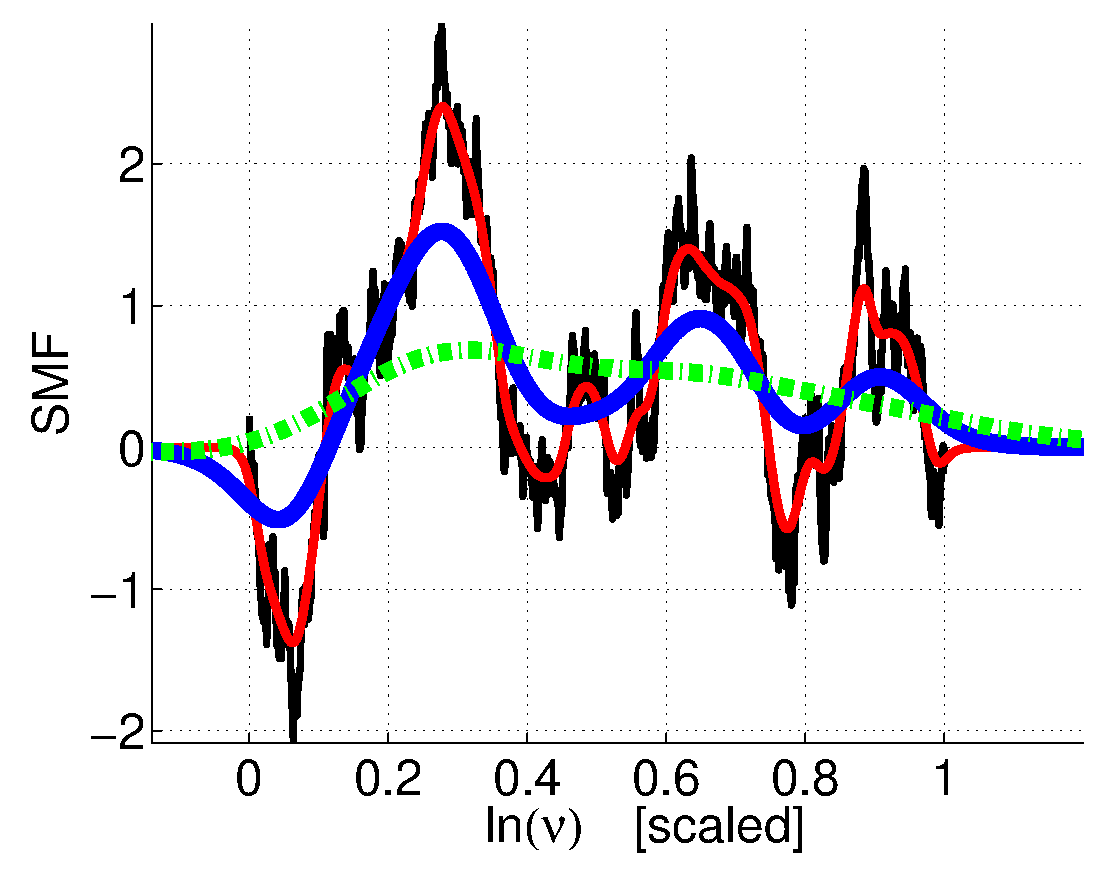
\includegraphics[width=6cm]{SMF_RW.eps}
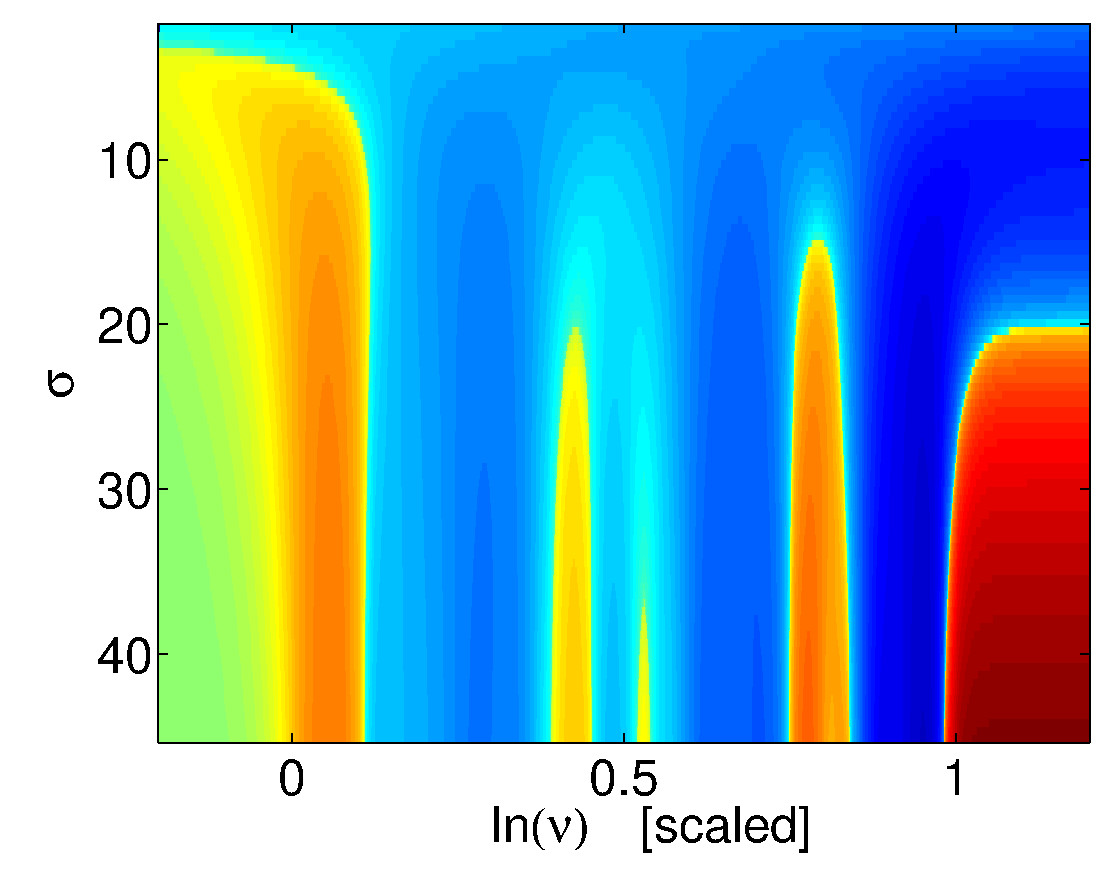
\includegraphics[width=6cm]{I_sig_tau.eps}

\caption{
We consider a ring with ${N=1000}$ sites whose energies 
are normally distributed with dispersion ${\Delta=1}$.
The bath temperature is $T_B=10$. In the upper panel 
the SMF of \Eq{e102} is plotted for $\sigma=\infty$, 
and for $\sigma=50,10,4$. The smaller $\sigma$, 
the smoother $\nu$ dependence. 
This is reflected in the current (lower panel).  
The horizontal axis is the scale $\ln(\nu)$ as defined in \Eq{e1021}.} 
\label{f2}
\end{figure}
%%%%%%%%%%%%%%%%%%%%%%%%%%%%%%



%%%%%%%%%%%%%%%%%%%%%%%%%%%%%%
\begin{figure}
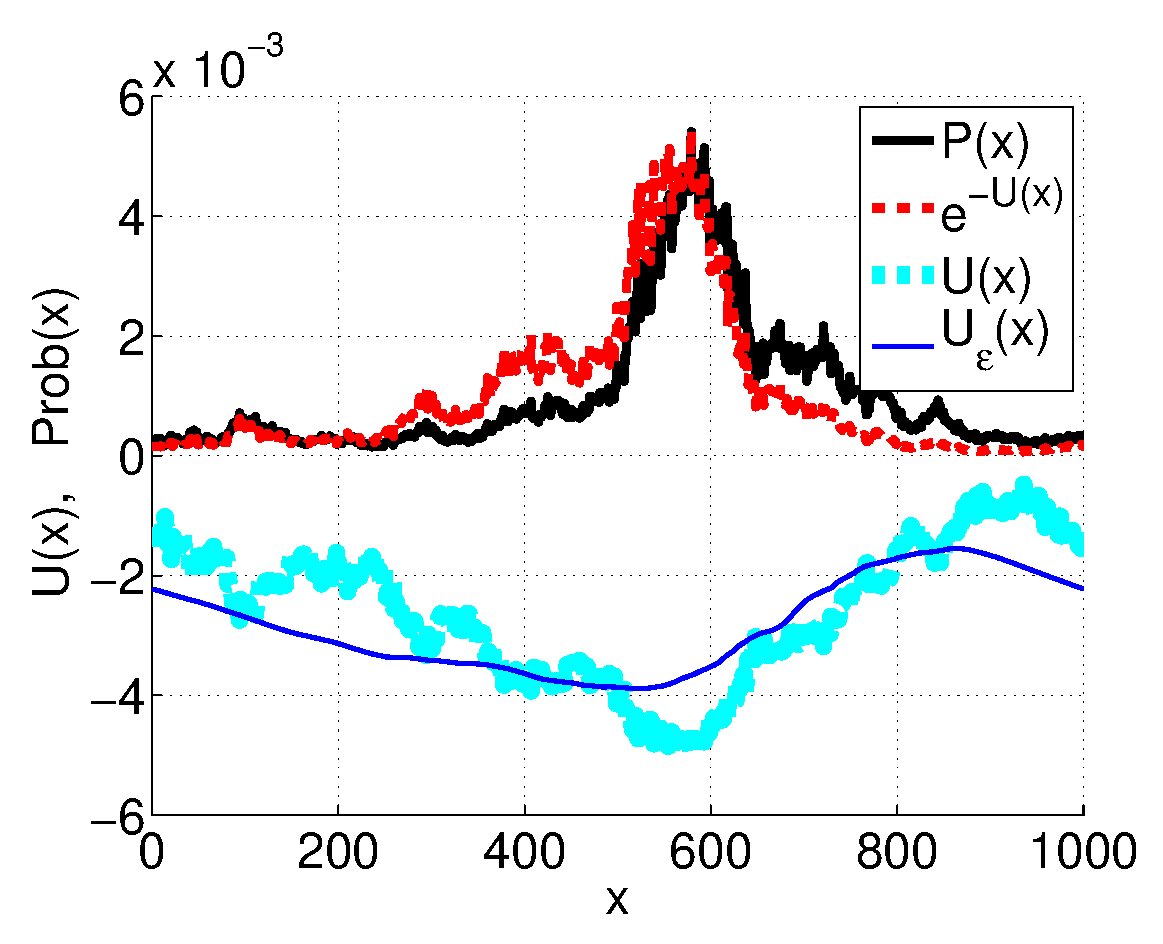
\includegraphics[width=7cm]{PvsV4}

\caption{
The NESS distribution of \Eq{e17} (solid black) 
is similar but not identical to the quasi-equilibrium 
distribution (dashed red line). 
Also shown, in the background is the potential 
landscape $U(x)$ and its smoothed version \rmrk{$U_{\varepsilon}(x)$}. 
The parameters as the same as in \Fig{f2}, 
however the bonds were rearranged to have a larger SMF, $\mathcal{E}_{\circlearrowleft}=7.4$.
The driving intensity \rmrk{corresponds to $\tau=0.3$}. }

\label{f3}
\end{figure}
%%%%%%%%%%%%%%%%%%%%%%%%%%%%%%



%%%%%%%%%%%%%%%%%%%%%%%%%%%%%%%%%
\begin{figure}
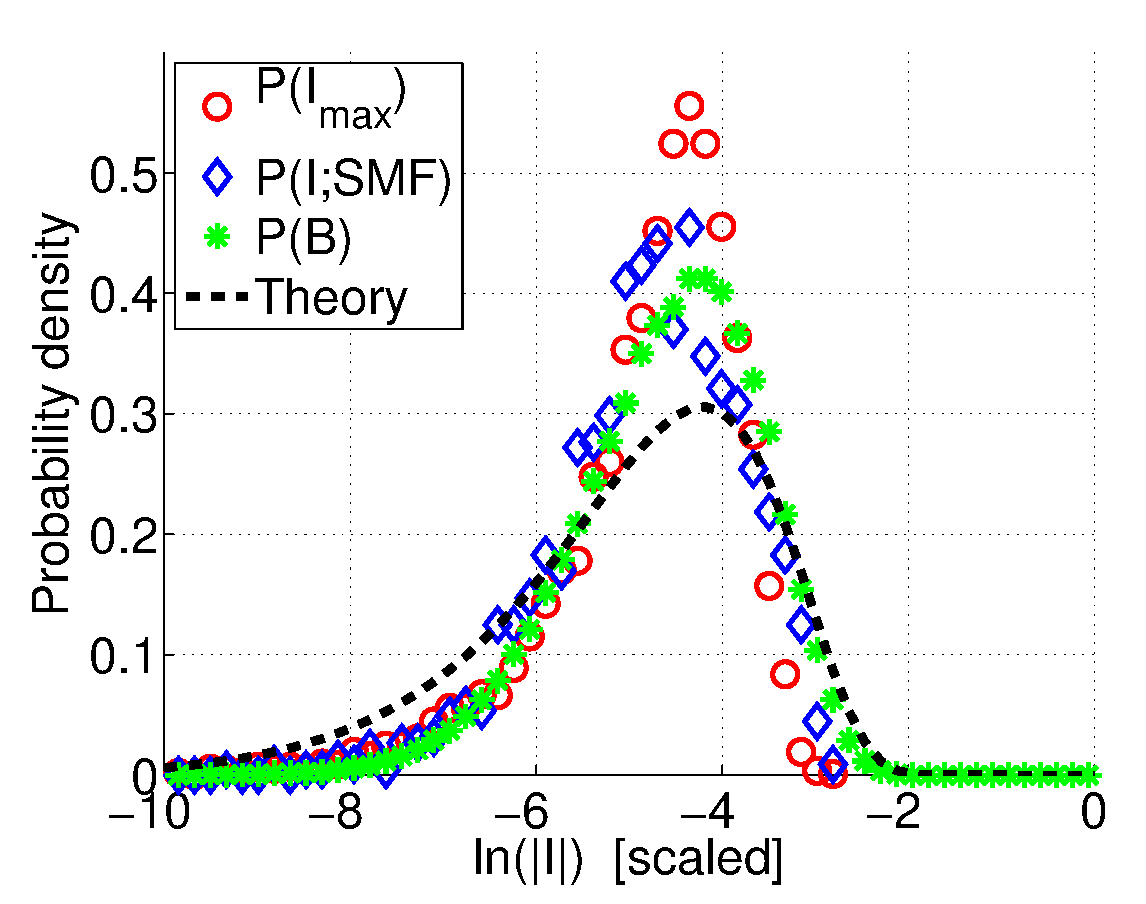
\includegraphics[width=6cm]{PlnI.eps}
%\begin{picture}(0,0)
%\put(-140,60){}
%\end{picture}

\vspace*{1cm}

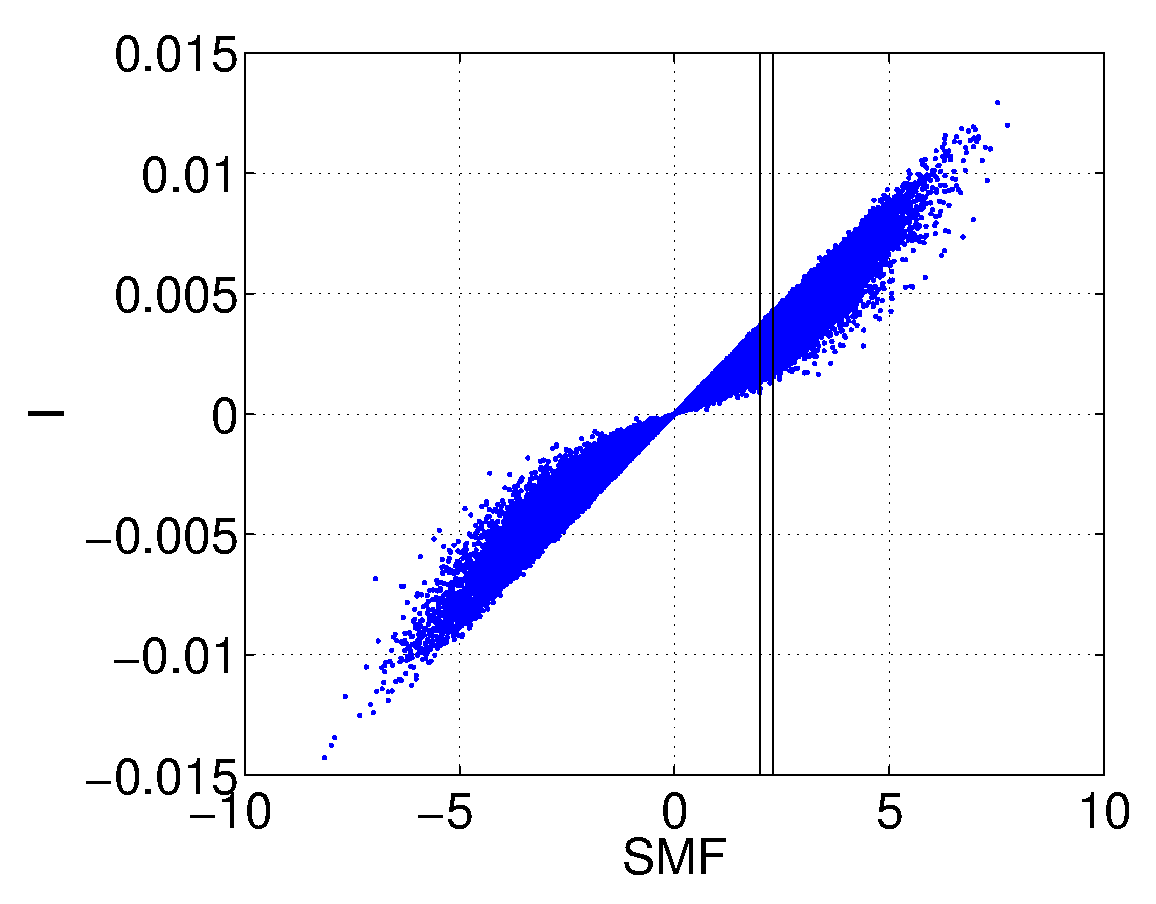
\includegraphics[width=6cm]{IvsSMF2.eps}

\vspace*{1cm}

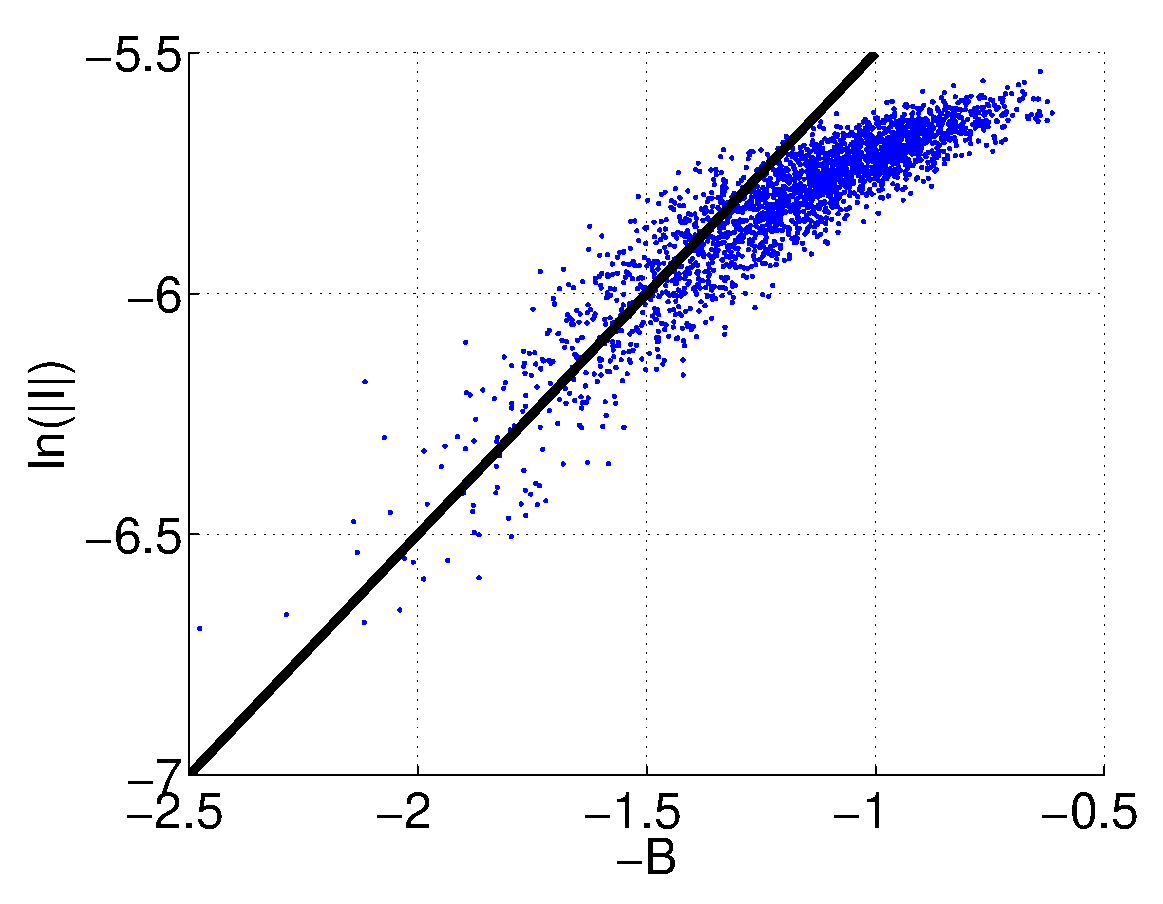
\includegraphics[width=6cm]{BvsLnI.eps}

\caption{Inset: scatter diagram of the current versus the SMF in the Sinai regime.
Note that in the linear regime, see \cite{SM}, it looks like a perfect linear 
correlation with negligible transverse dispersion. The distribution in the 
main upper panel corresponds to the slice ${\mathcal{E}_{\circlearrowleft} \in [2.0,2.1]}$. 
The long tails of small $I$ values reflects the likelihood of 
having a large activation barrier $B$. The lower panel displays the 
correlation between $I$ and $B$, hence the single-barrier approximation 
is established for small currents.}

\label{f4}
\end{figure}
%%%%%%%%%%%%%%%%%%%%%%%%%%%%%%%%%



%%%%%%%%%%%%%%%%%%%%%%%%%%%%%%%%%
\begin{figure}
\includegraphics[width=7cm]{CDFB.eps}
\begin{picture}(0,0)
%\put(-100,30){\includegraphics[width=3cm]{NES_Code/PB2.eps}}
\end{picture}

\caption{The cumulative distribution of $B$ compared with the analytical 
result of \Eq{e20}. There are no fitting parameters. 
The inset shows how the distribution density looks in normal scale. 
\rmrk{this is the most urgent action item}.}

\label{f5}
\end{figure}
%%%%%%%%%%%%%%%%%%%%%%%%%%%%%%%%%%%%%



%%%%%%%%%%%%%%%%%%%%%%%%%%%%%%%%%%%%%%%%%%%%%%%%%%%%%%%%%%%%%%%%%%%%%%%%%%%%%%%%%%%%
%%%%%%%%%%%%%%%%%%%%%%%%%%%%%%%%%%%%%%%%%%%%%%%%%%%%%%%%%%%%%%%%%%%%%%%%%%%%%%%%%%%%
\clearpage


%%%%%%%%%%%%%%%%%%%%%%%%%%%%%%%%%%%%%%%%%%%%%%%%%%%%%%%%%%%%%%%%%%%%%%%%%%%%
{\bf Acknowledgments.-- }
%
This research was supported by the Israel Science Foundation (grant No.29/11).
We thank Oleg Krichevsky (BGU) for a useful advice. SR is grateful for support from
the Israel Science Foundation (grant 924/11).


%%%%%%%%%%%%%%%%%%%%%%%%%%%%%%%%%%%%%%%
\begin{thebibliography}{99}

\bibitem{derrida}
B. Derrida, Y. Pomeau, 
% Classical Diffusion on a Random Chain
Phys. Rev. Lett. 48, 627 (1982).

\bibitem{d1}
S. H. Noskowicz, I. Goldhirsch,
% Average versus Typical Mean First-Passage Time in a Random Random Walk
Phys. Rev. Lett. 61, 500 (1988); 
% First-passage-time distribution in a random random walk
Phys. Rev. A 42, 2047 (1990). 

\bibitem{d2}
J. P. Bouchaud, A. Comtet, A. Georges, P. Le Doussal,
% Classical diffusion of a particle in a one-dimensional random force field 
Ann. Phys. (N.Y.) 201, 285 (1990).

\bibitem{d3}
H. E. Roman, M. Schwartz, A. Bunde, S. Havlin, 
% on fractals
Europhys. Lett. 7, 389 (1988). 

\bibitem{d4}
S.F. Burlatsky, G.S. Oshanin, A.V. Mogutov, M. Moreau,   
% Non-Fickian steady flux in a one-dimensional Sinai-type disordered system
Phys. Rev. A 45, R6955 (1992). 

\bibitem{sinai}
Ya. G. Sinai, 
Theory Probab. Appl. 27, 247 (1982).

\bibitem{sinai2}
S.F. Burlatsky, G.S. Oshanin, A.V. Mogutov, M. Moreau,   
% Non-Fickian steady flux in a one-dimensional Sinai-type disordered system
Phys. Rev. A 45, R6955 (1992). 



%%%%%%%%%%%%%%%%%%

\bibitem{surface}
R. L. Schwoebel and E. J. Shipsey, J. Appl. Phys. 37, 3682 (1966) 

\bibitem{brownian1}
M. O. Magnasco, Phys. Rev. Lett. 71, 1477 (1993) 

\bibitem{brownian2}
R. D. Astumian and M. Bier, Phys. Rev. Lett. 72, 1766 (1994)

\bibitem{brownian3}
M. O. Magnasco, Phys. Rev. Lett. 72, 2656 (1994)

\bibitem{ratchets}
P. Reimann, Phys. Rep. 361, 57 (2002)

\bibitem{motors1}
C.T. MacDonald, J.H. Gibbs and A.C. Pipkin, Biopolymers, 6, 1 (1968)

\bibitem{brownian4}
H. X. Zhou and Y. D. Chen, Phys. Rev. Lett. 77, 194 (1996) 

\bibitem{motors2}
E. Frey and K. Kroy, Ann. Phys. 14, 20 (2005)

\bibitem{motors3}
A.B. Kolomeisky and M.E. Fisher, Annu. Rev. Phys. Chem. 58, 675 (2007)

\bibitem{DNA1}
B. Xu, P. Zhang, X. Li and N. Tao, Nano Lett. 4, 1105 (2004)

\bibitem{DNA3}
H. W. Fink and C. Sch\"onenberger, Nature 398, 407 (1999)

%%%%%%%%%%%

\bibitem{Wichmann}
K. W. Kehr, K. Mussawisade, and T. Wichmann,
Phys. Rev. E 56, R2351 (1997).
% http://pre.aps.org/abstract/PRE/v56/i3/pR2351_1
% Rectification by hopping motion through nonsymmetric potentials with strong bias

\bibitem{Roling1}
A. Heuer, S. Murugavel, and B. Roling,
Phys. Rev. B 72, 174304 (2005).
% http://prb.aps.org/abstract/PRB/v72/i17/e174304
% Nonlinear ionic conductivity of thin solid electrolyte samples: Comparison between theory and experiment

\bibitem{Roling2}
S. Murugavel and B. Roling, 
J. Non-Cryst. Solids 351, 2819 (2005).

\bibitem{Roling3}
A. Heuer, S. Murugavel and B. Roling, 
Phys. Rev. B, 72, 174304 (2005).

\bibitem{Roling4}
B. Roling, S. Murugavel, A. Heuer, L. Luhning, R. Friedrich and S. Rothel, 
Phys. Chem. Chem. Phys. 10, 4211 (2008).

\bibitem{Nitzan}
M. Einax, M. Korner, P. Maass, A. Nitzan,
Phys. Chem. Chem. Phys. 12, 645 (2010).
% Nonlinear hopping transport %%%%%%%%%%%%%%%%%%%
in ring systems and open channels

%%%%%%%%%%%%%%%%%%%

\bibitem{kbb}
D. Hurowitz, D. Cohen,
Europhysics Letters 93, 60002 (2011) 


\bibitem{ner} 
D. Hurowitz, S. Rahav, D. Cohen,
%{\em The non-equilibrium steady state of sparse systems with non-trivial topology}. 
Europhysics Letters 98, 20002 (2012) 


%%%%%%%%%%%%%%%%%%%

\bibitem{eprd1} % entropy production
J.L. Lebowitz, H. Spohn, J. Stat. Mech, v95 333 (1999).

\bibitem{eprd2}
P. Gaspard, J. Chem. Phys., 120, 8898 (2004).

\bibitem{eprd3}
Udo Seifert, % Entropy Production along a Stochastic Trajectory and an Integral Fluctuation Theorem
Phys. Rev. Lett. 95, 040602 (2005)

\bibitem{eprd4}
D. Andrieux and P. Gaspard, J. Stat. Phys., 127, 107 (2007).




\bibitem{rw1}
Adrienne W. Kemp,
%The Moments of the Random Variable for the Number of Returns of a Simple Random Walk
Advances in Applied Probability , Vol. 19, No. 2 (Jun., 1987), pp. 505-507

\bibitem{feller}
W. Feller, 
An Introduction to Probability Theory and its Applications.

\bibitem{dwass}
%Simple Random Walk and Rank Order Statistics
Meyer Dwass,
The Annals of Mathematical Statistics , Vol. 38, No. 4 (Aug., 1967), pp. 1042-1053
\rmrk{not cited}



\bibitem{net1}
J. Schnakenberg,
% Network theory of microscopic and macroscopic behavior of master equation systems
Rev. Mod. Phys. 48, 571 (1976).

\bibitem{net2}
T.L. Hill, 
J. Theor. Biol. v10, 442 (1966)

\bibitem{net3}
R.K.P. Zia, B. Schmittmann, 
J. Stat. Mech., P07012 (2007).

\bibitem{DNA2}
P. Kohli, C. C. Harell, Z. Cao, R. Gasparac and R. Martin, Science 305, 984 (2004).


%%%%%%%%%%%%%%%%%


\bibitem[a]{images}
This illustration combines pieces of images 
that were taken from \rmrk{URL} and \rmrk{URL}.

\bibitem[b]{SM}
See supplementary material at URL for some extra technical details \rmrk{regarding...}

%%%%%%%%%%%%%%%%%%%%%%%%%

\ \\ \ \\ 

%%%%%%%%%%%%%%%%%%%%%%%%%

\bibitem{saar} 
\rmrk{From here on excluded unless intro is modified.}
I.M. Sokolov and A. Blumen, J. Phys. A 30, 3021 (1997). 
S. Rahav, J. Horowitz, C. Jarzynski,
%{\em Directed Flow in Nonadiabatic Stochastic Pumps}. 
Phys. Rev. Lett. 101, 140602 (2008)

\bibitem{Saar}
S. Rahav, J. Horowitz, C. Jarzynski,
%Directed flow in nonadiabatic stochastic pumps,
Phys. Rev. Lett., 101, 140602 (2008).

\bibitem{st1}
D. A. Leigh,  J.K.Y. Wong, F. Dehez, F. Zerbetto,
% Unidirectional rotation in a mechanically interlocked molecular rotor
Nature (London) 424, 174 (2003)

\bibitem{st2}
J.M.R. Parrondo,
% Reversible ratchets as Brownian particles in an adiabatically changing periodic potential
Phys. Rev. E 57, 7297 (1998)

\bibitem{st4}
R.D. Astumian,
% Stochastic conformational pumping: a mechanism for free-energy transduction by molecules.
Annu Rev Biophys.40, 289-313 (2011)


\end{thebibliography}


%%%%%%%%%%%%%%%%%%%%%%%%%%%%%%%%%%%%%%%%%%%%%%%%%%%%%%%%%%%%%%%%%%%%%%%%%%%%%%%%%%%%%

\clearpage
\onecolumngrid

\begin{center}
{\LARGE\bf Supplementary Material}
\end{center}

%\twocolumngrid


%%%%%%%%%%%%%%%%%%%%%%%%%%%%%%%%%%%%%%%%%%%%%%%%%%%%%%%%%%%%%%%%%%%%%%%%%%%%%%%%%%%%
\section{Detailed definition of the model}

Including detailed explanation of Eq(2) 

Form the detailed balance condition it follows that 
to leading order 
%
\beq
w^{\beta}_{\overrightarrow{n}} \ &\approx& \ \left[1-\frac{1}{2}\left(\frac{E_n-E_{n{-}1}}{T_B}\right)\right]\bar{w}_{\bar{n}}^{\beta} \\ 
w^{\beta}_{\overleftarrow{n}} \ &\approx& \ \left[1+\frac{1}{2}\left(\frac{E_n-E_{n{-}1}}{T_B}\right)\right]\bar{w}_{\bar{n}}^{\beta}
\eeq  
%
It follows that 
%
\beq
\frac{w_{\overrightarrow{n}}}{w_{\overleftarrow{n}}} 
\ \ = \ \ \frac{w^{\beta}_{\overrightarrow{n}}+\nu g_{\bar{n}}}{w^{\beta}_{\overleftarrow{n}}+\nu g_{\bar{n}}}
\ \ \approx \ \ 1+ \frac{(E_n-E_{n{-}1})/T_B}{1+(g_{\bar{n}}/\bar{w}_{\bar{n}}^{\beta})\nu}
\eeq
%
Absorbing the bath couplings into the definition of the $g_{\bar{n}}$ we get  
%
\be{1001}
\mathcal{E}(x_n) \ \equiv \ \ln \left[\frac{w_{\overrightarrow{n}}}{w_{\overleftarrow{n}}}\right] 
\ \approx \ - \left[ \frac{1}{1+g_{\bar{n}}\nu} \right] \frac{E_n{-}E_{n{-}1}}{T_B}
\ee

%%%%%%%%%%%%%%%%%%%%%%%%%%%%%%%%%%%%%%
\section{Definition of regimes}

There are 3 regimes, depending on the driving intensity and sparsity
% 
\beq
\text{Linear}&:& \ \nu < g_{max}^{-1} \\
\text{Sinai}&:&  \ g_{max}^{-1} < \nu < g_{min}^{-1}\\
\text{Saturation}&:& \ \nu > g_{min}^{-1}
\eeq
%
The main body of the paper dealt with the Sinai regime.
In the linear and saturation regimes, it is possible to obtain 
expressions for the current and SMF. To calculate the SMF, we integrate  \Eq{e1001} along the entire ring 
%
\be{-1}
\mathcal{E}_{\circlearrowleft} 
\approx  -\sum_{n=1}^N \left[ \frac{1}{1+g_{\bar{n}}\nu} \right] \frac{\Delta_n}{T_B}
\eeq



Recall that we have ${\sum_n\Delta_n=0}$. Additionally we define 
%
\beq
\Delta^{(0)} &\equiv&  \sum_{n} g_{\bar{n}}  \Delta_n 
\ \sim \ \pm \Big[2N \, \mbox{Var}(g)\Big]^{1/2} \Delta
\\
\Delta^{(\infty)} &\equiv& \sum_{n} \frac{1}{g_{\bar{n}}}  \Delta_n
\ \sim \ \pm \Big[2N \, \mbox{Var}(g^{-1})\Big]^{1/2} \Delta
\eeq
%
The RMS-based estimate of the sums follows from the observation 
that, say, $\Delta^{(0)}$ can be rearranged as 
${\sum_n (g_{\bar{n}+1}-g_{\bar{n}}) E_n}$, 
which is a sum of~$N$ independent random variables.  
Consequently we get for the SMF the following approximation 
%
\be{131}
\mathcal{E}_{\circlearrowleft} \ \ \approx \ \ 
\frac{1}{T_B}
\left\{
\amatrix{
\Delta^{(0)}\nu, & \ \ \text{Linear} \cr 
-\Delta^{(\infty)}/\nu , & \ \ \text{Saturation}
}\right.
\eeq
%
since  $\Delta^{(0)} $ and $\Delta^{(\infty)} $ 
are both sums of independent random variables,
they may be expected to behave according to the central limit theorem.
This is verified in \Fig{f6}, 
where it is shown that  $\Delta_0$ follows a normal distribution.


%The current may be approximated as 
%%
%\be{55}
%I \approx \frac{1}{N} \left\{\begin{array}{cc}
%-\frac{\Delta^{(0)}}{T_B} w^{\nu}, & \ \text{linear regime}\\
%\frac{\Delta^{(\infty)}}{T_B} w^{\beta}, & \  \text{Saturation}\end{array}\right.
%\ee
%%

%%%%%%%%%%%%%%%%%%%%%%%%%%%%%%%%%%%%%%%%%%%%%%%%%%5
\section{More details on serial addition}

e.g. expression for $\overleftarrow{G}$ analogous to Eq(8).

%%%%%%%%%%%%%%%%%%%%%%%%%%%%%%%%%%%%%%%%%%%%%%%%%%
\section{Statistics related to random walk}

Naively, one might think that the distribution of $I$ 
is determined by the maxima of the energy landscape $\mathsf{max}\{U(x)\}$.
To test this hypothesis, we notice first that $\mathsf{max}\{U(x)\}$ is the same as the point furthest from the origin that a random walker reaches.
The distribution of this extreme point $K$ in random walk of $N$ steps is given by (see for example \cite{dwass})
%
\beq
P(K \geq k;N) &=&  \left(\begin{array}{c}2N \\N-k\end{array}\right) / 
\left(\begin{array}{c}2N \\N\end{array}\right),  \\ 
k &=& 0,1,2\cdots N
\eeq
%
Switching variables to $u=k/N$ and taking the large $N$ limit, 
one obtains the probability distribution function $P(\mathsf{max}\{U\} =u) = f(u)$
%
\be{50}
 f(u) = \ln \left[\frac{1+u}{1-u} \right] \left[\frac{(1-u)^{u-1}}{(1+u)^{u+1}}\right]^N \frac{N}{1-4^{-N}} 
\ee
%
Which has a peak at $u=1/\sqrt{2N}$.
For values $u\ll1$, this expression can be approximated by the simple function
%
\be{51}
f(u) \approx 2ue^{-Nu^2} \frac{N}{1-e^{-N}}, \ u\geq 0
\ee
%
In \Fig{pu} we plot \Eq{e50}, \Eq{e51} and the maxima of $U(x)$.
%
\begin{figure}
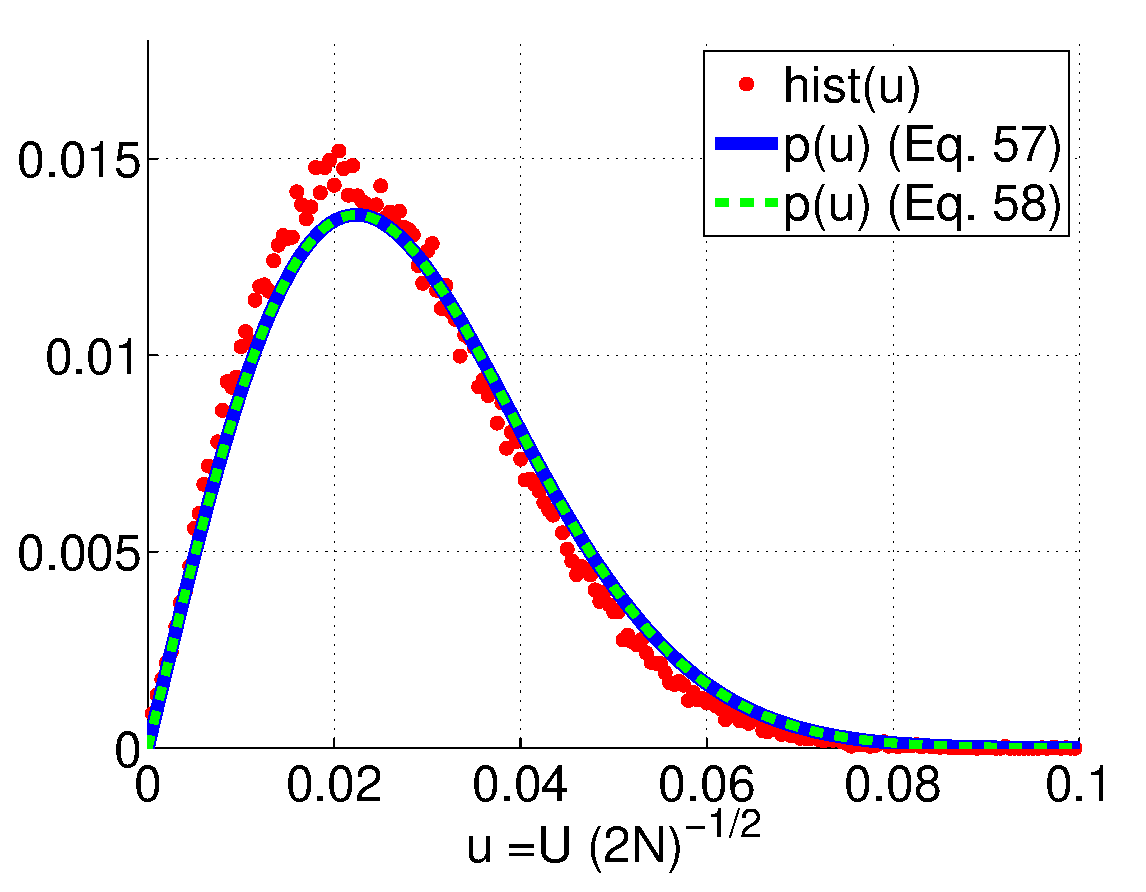
\includegraphics[width=6cm]{PmaxV.eps} 
\caption{
Histogram of maxima of $u=\mathsf{max}\{U(x)\}$ (red points) and distribution of maxima of random walk (blue line) of equivalent length, \Eq{e50}. Also shown is the approximation, \Eq{e51} which holds for the region of interest.
}
\label{pu}
\end{figure}
%
\begin{figure}
\includegraphics[width=6cm]{PB.eps}
\caption{
Histogram of barriers (red points) and naive distribution of barriers in a random walk (blue line) of equivalent length, \Eq{e52}. }
 \label{pb}
\end{figure}

%%%%%%%%%%%%%%%%%%%%%%%%%%%%%%%%%%%%%%%%%%%%%%%%%%
\section{Derivation of the $B$ statistics}

The derivation of the distribution of barrier heights is as follows.
We consider a random walk of $N$ steps, $Y(N) = X_1+X_2+\cdots X_N$ 
and calculate the survival probability within the boundaries $x_a,x_b$:
\beq
\text{Prob}\left(x_a<Y(N) <x_b\right) 
\eeq
The joint probability distribution of extreme points is
\beq
f(x_a,x_b) = -\frac{d}{dx_a}\frac{d}{dx_b}P
\eeq
Define the barrier $R$ and center of mass $X$ via the 
coordinate transformation 
\beq
R &=& \frac{x_a+x_b}{2} \\
X &=& x_b-x_a
\eeq
So $dXdR=d{x_a} d {x_b}$.
The distribution of barriers is obtained by calculating the 
marginal distribution
\beq
f(R) &=&- \int_{-\infty}^{\infty}dx_a \int_{x_a}^{\infty} dx_b f(x_a,x_b)\delta\left( R - (x_b-x_a)\right)\\
&=& -\int_{0}^{\infty}dR' \int_{0}^{R'} dX f(X,R') \delta (R-R') = \int_{0}^{R} f(R,X)dX = \\
&=& - \int_{0}^{R} (\frac{1}{4}\partial_X^2-\partial_R^2)P_t(R,X)dX=\\
&=&  \int_{0}^{R} \partial_R^2P_t(R,X)dX=\\
%&=&  -\int_{-R/2}^{R/2} \partial_R^2P_t(R|X)P(X)dX=   -\int_{-R/2}^{R/2} \partial_R^2P_t(R|X)\frac{X}{R}dX=\\
&=& \partial_R^2 R P_t(R|\text{uniform})
%&=&  -\int_{-R/2}^{R/2} \partial_R^2P_t(X|R)P(R)dX=
\eeq
In the last step we use the fact that (a) $P_t(R,X=0)=P_t(R,X=R)=0$ and (b) the linearity of the diffusion equation: instead of calculating $P_t(R,x)$ for various initial points $x$ and summing over $x$, we solve 
for an initially uniform distribution
\beq
P_t(R|\text{uniform}) = \rho_t(x), \ \ \rho_{t=0}(x)=\frac{1}{R}
\eeq
Where $\rho_t(x)$ is the solution to the 1D diffusion equation on the interval $[0,R]$:
\beq
\rho_t(x) = \sum_{n=1,3,5,...}^{\infty} \exp\left[-D \left(\frac{\pi n}{R}\right)^2t\right]  A_n \sin(\frac{\pi n}{R}x)
\eeq
Starting with a uniform distribution $\rho_0(x)=1/R$, we obtain the coefficients $A_n$
\beq
\rho_t(x) = \sum_{n=1,3,5,...}^{\infty} \exp\left[-D \left(\frac{\pi n}{R}\right)^2t\right] \frac{4}{\pi n R}\sin(\frac{\pi n}{R}x)
\eeq
So the survival probability within a region $R$, given an initially uniform distribution, is
\beq
P_t(R|\text{uniform}) = \int_{0}^{R} \rho_t(x)dx =  
\sum_{n=1,3,5,...}^{\infty} \exp\left[-D \left(\frac{\pi n}{R}\right)^2t\right] \frac{8}{\pi^2 n^2 }
\eeq
And we get for $f(R)$
\beq
f(R)  &=&    \frac{\partial^2}{\partial R^2} R \sum_{n=1,3,5,...}^{\infty} \exp\left[-D \left(\frac{\pi n}{R}\right)^2t\right] \frac{8}{\pi^2 n^2 }
\eeq
The sum may be approximated by an integral (\Fig{f8}):
\beq
 P_t(R|\text{uniform})  &=& \sum_{n=1,3,5,...}^{\infty} \frac{1}{n^2}\exp\left[-\frac{\alpha}{R^2}n^2 \right] 
  \approx \frac{1}{2} \int_1^{\infty}  \frac{1}{x^2} \exp\left[-\frac{\alpha}{R^2}x^2 \right] dx = \\
&=&  \exp \left(-\frac{\alpha}{R^2} \right)-\sqrt{\pi\frac{\alpha}{R^2}}  \mathsf{erfc}\left(\sqrt{\frac{\alpha}{R^2}} \right)  \eeq
 Where $\alpha=\pi^2Dt$. 
%We realise that this maybe written as a parametric derivative:
%\beq
%F(\lambda) &=& \int_1^{\infty}  \frac{1}{x^2} e^{-\lambda x^2} dx\\
%F'(\lambda) &=& - \int_1^{\infty} e^{-\lambda x^2 }dx = -\frac{\sqrt{\pi}}{2}\mathsf{erfc}
%\left(\sqrt{\lambda}\right)
%\eeq
Finally,
\beq
f(R) %&=& - \frac{8R}{\pi^2} \frac{\partial^2}{\partial R^2}  F \left({\frac{\alpha}{R^2}}\right) = \\
&=&   \frac{2}{\pi^2} \frac{\partial^2}{\partial R^2} \left[ R \int_1^{\infty}  \frac{1}{x^2} \exp\left(-\frac{\alpha}{R^2}x^2 \right) \right]dx\\
&=&\frac{2}{\pi^2} \frac{2\alpha}{R^3}\exp\left(-\frac{\alpha}{R^2} \right)
%\int_1^{\infty}  \frac{2\alpha}{R^3} \exp\left[-\frac{\alpha}{R^2}x^2 \right] dx\\
%&=&   \frac{4\alpha}{\pi^{3/2}}  \frac{\partial}{\partial R}   \left[ \frac{1}{R^2} \mathsf{erfc}\left(\sqrt{\frac{\alpha}{R^2}} \right) \right] \\
%&=& -2\alpha \frac{\partial}{\partial R} \left[ \frac{1}{R^3}   F' \left({\frac{\alpha}{R^2}}\right)\right]
\eeq
And the CDF is 
\beq
P(\text{barrier}<R)=\exp\left(-\frac{\pi^2DN}{R^2}\right)
\eeq
\begin{figure}
\includegraphics[width=8cm]{Pt.eps}
\caption{
The function increases from zero to 1, however for small $R$, the function is convex while for large $R$ it is concave, so $f(R$) changes sign...
}
\label{f8}
\end{figure}


%%%%%%%%%%%%%%%%%%%%%%%%%%%%%%%%%%%%%%%%
\clearpage
\begin{figure}
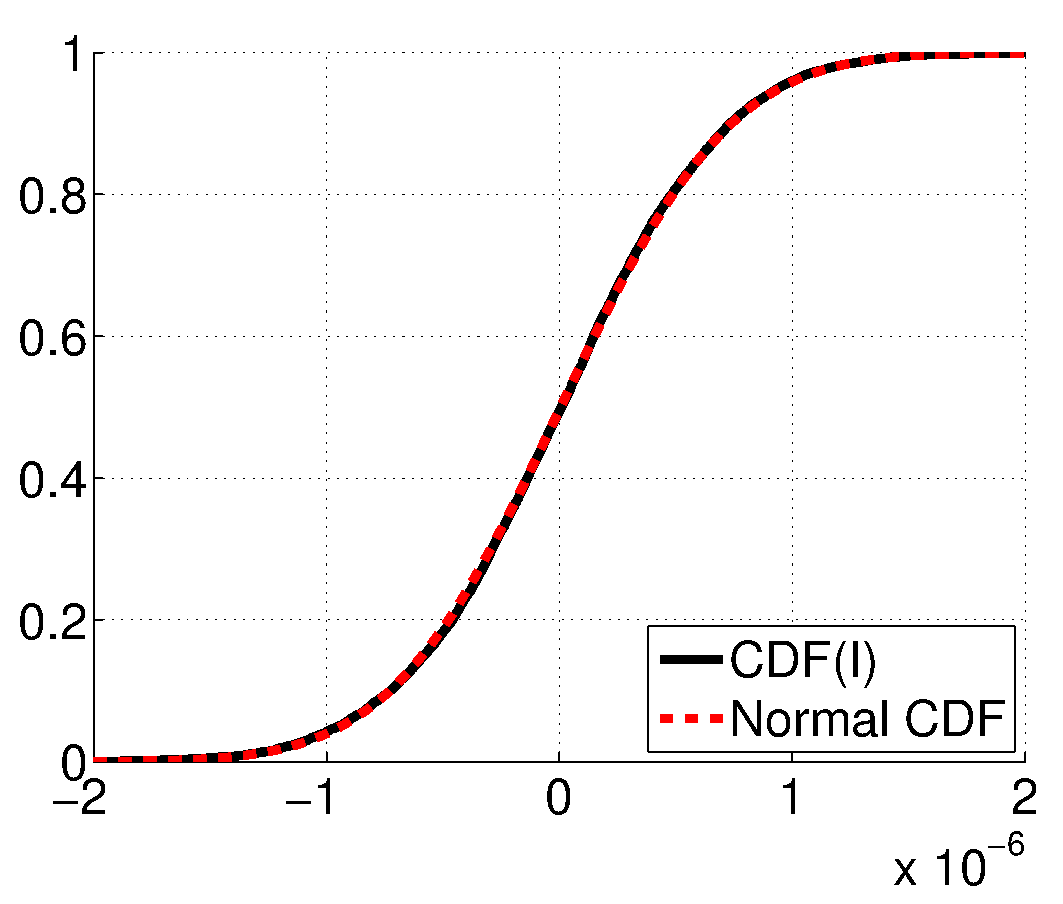
\includegraphics[width=8cm]{lin1.eps}%
\begin{picture}(0,0)
\put(-210,100){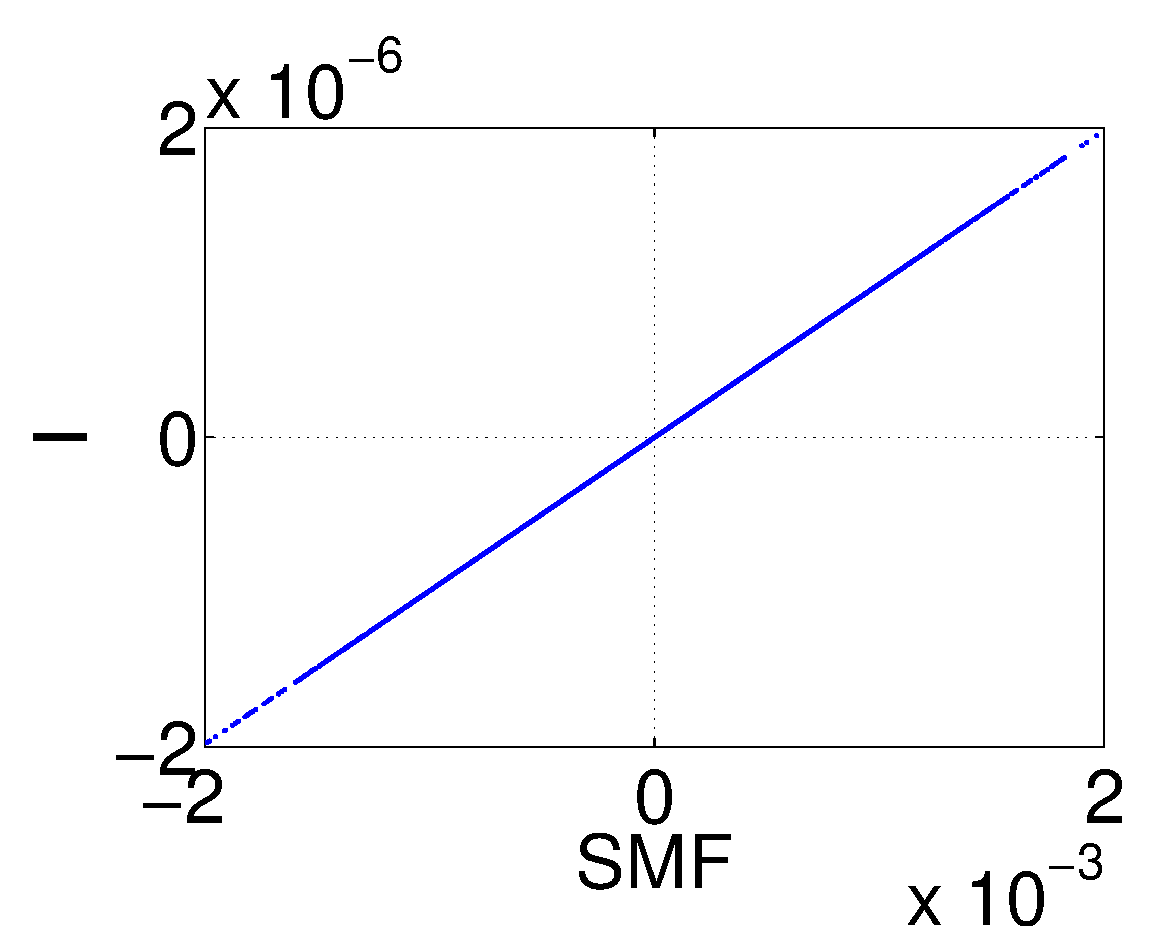
\includegraphics[width=3.5cm]{lin2.eps}}
\end{picture}
\caption{
In the linear regime, the current has a normal distribution. Since,
${I \propto w_{\epsilon} \mathcal{E}_{\circlearrowleft}}$, 
for a given value of $ \mathcal{E}_{\circlearrowleft}$ the dispersion is very small (scatter plot of current vs. SMF in the inset)
due to the central limit theorem.
For the statistical analysis we generated $10^5$ realisations with $\sigma=6$. 
}
\label{f6}
\end{figure}
%%%%%%%%%%%%%%%%%%%%%%%%%%%%%%%%%



\end{document}

















